\section{Introduction}

The aim of this design is to eliminate the use of the genesis keys (or delegates) within the formal ledger rules.  This will enable
decentralised governance of the blockchain protocol by supporting automated submission and enactment of proposals (PUP).
The process is designed to meet current and future national and international regulatory concerns by removing control of the blockchain protocol
from a small centralised group of actors.

There are three places where genesis keys are currently used.


\begin{itemize}
\item
  \textbf{Parameter Updates:}
  Any updatable protocol parameter may be changed.  Multiple parameters may be changed as part of a single update proposal.
\item
  \textbf{Protocol Version Changes:}
  A change may be made to a major or minor protocol version (a ``hard fork'').  The change must be accompanied by upgrades to
  the software that is being used by block producing nodes (``stake pools''), and acknowledged by sufficient pools upgrading to the new software version.
\item
  \textbf{Transfers from/to Reserves/Treasury:}
  A funds transfer may be made directly from eiher the reserves or treasury pots to a nomrmal address, between the reserves and treasury pots (in either direction), or from a normal address to the treasury pot.  This is referred to in the existing Cardano documentation as an ``MIR'' transfer (Move Instantaneous Rewards).
\end{itemize}

All of these must be devolved to a decentralised governance process.

\subsection{Outline Governance Process}

The governance process involves both off-chain and on-chain components.

\begin{enumerate}
\item
  \textbf{Off-Chain:}
  An issue is discussed off-chain.  A vote is taken on a specific proposal using the Catalyst system.  The proposal must be sufficiently unambiguous that its intention is clear, and must include dates by which the proposal is to be submitted and enacted on chain.
\item
  \textbf{On-Chain:}
  A formal proposal is constructed that captures the intention of the off-chain proposal.  It is submitted, verified, and then enacted on-chain.  The proposal will include a date by which it must be enacted.
\end{enumerate}


The outline process is shown in Figure~\ref{fig:workflows}.   The process is split into two main parts: the initial off-chain process, which is largely manual; and the second, on-chain process, which is largely
automated.  Only the latter needs to be captured by formal ledger rules.  It is necessary to

\begin{figure}
  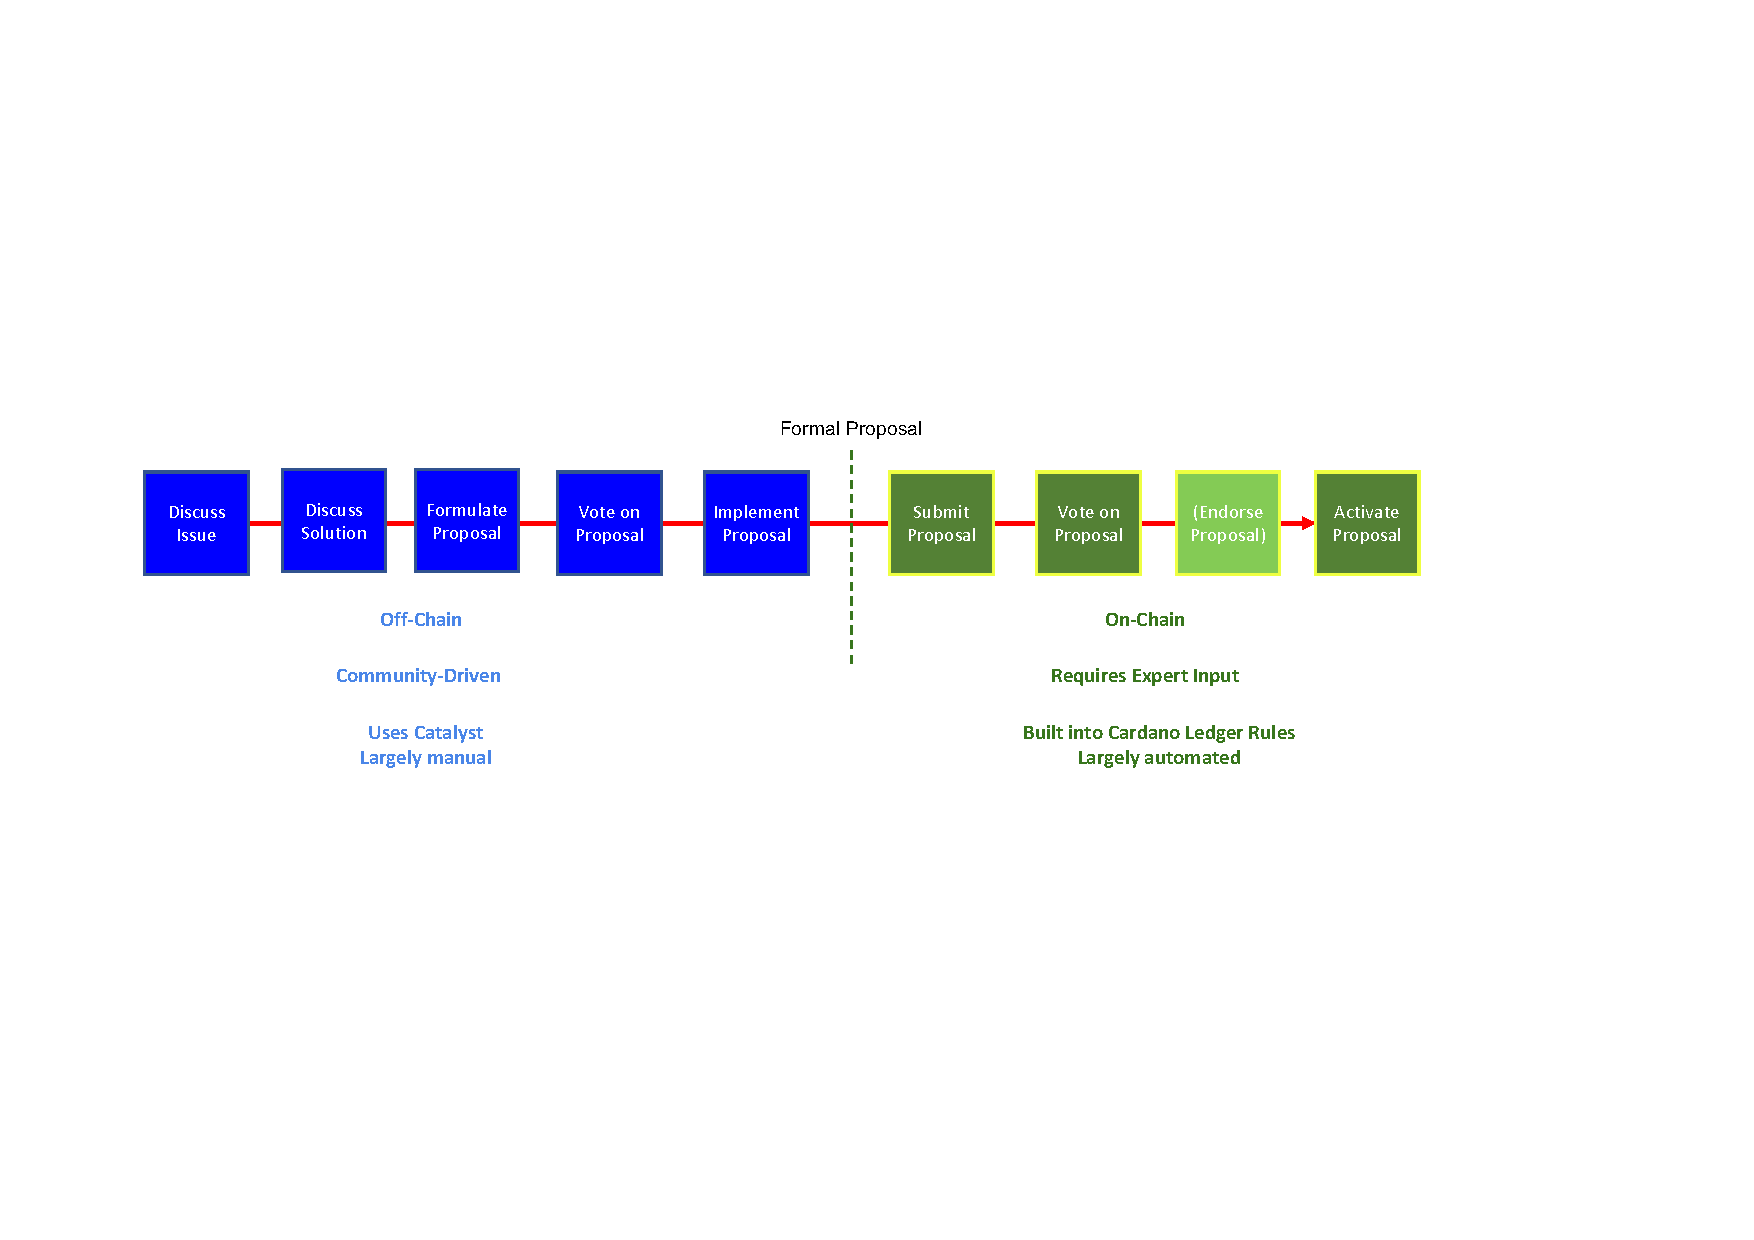
\includegraphics[trim=30 200 100 100,clip,width=\textwidth]{StoryBoard}
  \caption{Outline Process: Ideas are discussed off-chain and voted on using the Catalyst mechanism.  Successful proposals are implemented, and then submitted for on-chain voting and enactment.}
\label{fig:workflows}
\end{figure}


\subsection{Off-Chain Process}

The off-chain process involves five key stages:

\begin{enumerate}
\item
  \textbf{Discussion.}  An issue is discussed informally.
\item
  \textbf{Ideation.}  A concrete proposal that addresses the issue is formulated by an interested party.
\item
  \textbf{Submission.}  A proposal is submitted for voting.
\item
  \textbf{Voting.}  Voters may vote on whether a proposal should be progressed to implementation, requires amendment etc.  Outline deadlines should be agreed.
\item
  \textbf{Implementation.}  Accepted proposals are implemented.  For a simple proposal (eg a change to an updatable parameter), this may be as simple as capturing the intentions of the original proposal in a corresponding JSON file.
\end{enumerate}

These off-chain stages may follow formally defined processes, and be partially automated.  Generally, they will driven by convention and rules.  A detailed governance structure is necessary to ensure that necessary business can
be transacted in an efficient and effective way, without risking loss of control to a small non-representative group.


\subsection{On-Chain Process}

Once a proposal has been implemented, it may be submitted for enactment on-chain.  The on-chain process involves four key stages that are fully automated.  Extreme care needs to be taken with these processes,
since it may not always be possible to stop or reverse actions once they are initiated.

\begin{enumerate}
\item
  \textbf{Submission.}  A formal proposal is submitted on-chain by one of a group of submitters.  The proposal must be in the agreed format, and must include deadlines for voting and enactment.
\item
  \textbf{Voting.}  The proposal is voted on and the votes are tallied.  If sufficient votes are obtained by the stated deadline, then the proposal is approved for enactment.
\item
  \textbf{Endorsement.}  If the proposal involves a change to the protocol, then stake pool operators must upgrade their node to the correct version.  This will signal their readiness to run the new protocol.
  If sufficient endorsement is obtained by the deadline, then the proposal is endorsed for enactment.
\item
  \textbf{Enactment.}  Proposals that have been approved (and endorsed, if necessary) are processed fully automatically at the correspponding epoch boundary.
\end{enumerate}

\newpage
\subsection{Key Stakeholder Groups}

The key stakeholder groups are:

\begin{itemize}
\item
  \textbf{Normal Ada Holders:}
  Normal Ada holders are invested in the Cardano ecosystem in financial and other ways.
  The goal is for them to have the ultimate governance power, but they may choose to delegate this to specialists when dealing with more technical issues, for example.
  This ensures fully decentralised governance.
  \item
  \textbf{Stake Pool Operators:}
  Stake pool operators have the responsibility for maintaining the Cardano network.  They need to maintain compatibility with the latest version of the Cardano blockchain protocol.
  \item
  \textbf{End-Users:}
  Individuals or organisations who are using the Cardano blockchain to process transactions etc.  They may hold minimal ada on a transient basis, which will give them limited or no governance rights.
  \item
  \textbf{Exchanges and other Proxy Ada Holders:}
  Exchanges and similar organisations hold Ada on behalf of other parties.  It is important from a regulatory and technical perspective that they do not hold excessive
  power, since this will work against the requirements of decentralisation.
\end{itemize}

The network should be able to evolve in a way that meets the best long-term needs of all these stakeholders, while maintaining the integrity, stability and longevity of
the Cardano blockchain.
